\documentclass[tikz,border=6pt]{standalone}
\usepackage{tikz}

\begin{document}
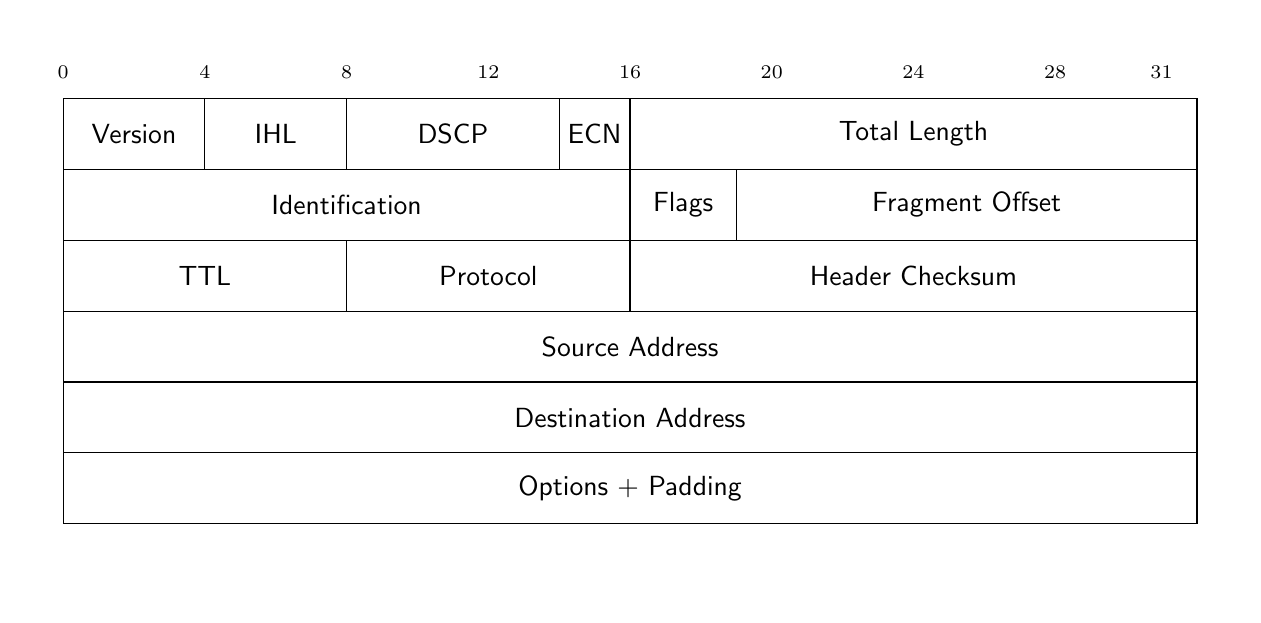
\begin{tikzpicture}[
  x=0.45cm,
  y=0.9cm,
  font=\sffamily,
  bitlabel/.style={font=\scriptsize}
]

% White background
\fill[white] (-1,-1) rectangle (33,7);

% Bit positions
\foreach \x/\lbl in {0/0,4/4,8/8,12/12,16/16,20/20,24/24,28/28,31/31} {
  \node[bitlabel, anchor=south] at (\x,6.15) {\lbl};
}

% Grid rows
\foreach \y in {0,1,2,3,4,5} {
  \draw (0,\y) rectangle (32,\y+1);
}

% Vertical splits
\draw (4,5) -- (4,6);
\draw (8,5) -- (8,6);
\draw (14,5) -- (14,6);
\draw (16,5) -- (16,6);

\draw (16,4) -- (16,5);
\draw (19,4) -- (19,5);

\draw (8,3) -- (8,4);
\draw (16,3) -- (16,4);

% Labels
\node at (2,5.5) {Version};
\node at (6,5.5) {IHL};
\node at (11,5.5) {DSCP};
\node at (15,5.5) {ECN};
\node at (24,5.5) {Total Length};

\node at (8,4.5) {Identification};
\node at (17.5,4.5) {Flags};
\node at (25.5,4.5) {Fragment Offset};

\node at (4,3.5) {TTL};
\node at (12,3.5) {Protocol};
\node at (24,3.5) {Header Checksum};

\node at (16,2.5) {Source Address};
\node at (16,1.5) {Destination Address};
\node at (16,0.5) {Options + Padding};

\end{tikzpicture}
\end{document}